\documentclass[openany,12pt,a4paper]{report}
\usepackage{subfiles}
\usepackage[numberedsection]{glossaries}
\usepackage[]{graphicx}
\usepackage{float}
\usepackage{multirow}
\graphicspath{{./img/}{./../img/}}
\usepackage{../StileDoc}
\title{Manuale Utente}
\author{}

%Ultima versione documento
\newcommand{\versione}{1.0.0}

% Stile per il glossario
\newglossarystyle{glossaryStyle}{
	\setglossarystyle{altlistgroup}
	\renewcommand*{\glsgroupheading}[1]{
		% Tolgo la numerazione per l'indice
		\setcounter{secnumdepth}{0}
		\section{##1}
		\vspace*{-\baselineskip}
		% Solo per fare un po' di spazio tra la lettera e le voci
		\item\makebox[\linewidth]{\hspace*{2cm}}
	}
}

\glsaddall

\makeglossaries

%Term definitions
\newglossaryentry{Speect}{name=Speect, description={Libreria di Text-To-Speech di riferimento per il progetto DeSpeect}}
\newglossaryentry{GCC}{name=GCC, description={Compilatore C++ di riferimento per il progetto DeSpeect}}
\newglossaryentry{GitHub}{name=GitHub, description={Servizio di versionamento per progetti software}}
\newglossaryentry{Qt}{name=Qt, description={Libreria multipiattaforma per lo sviluppo di programmi con interfaccia grafica tramite l'uso di widget}}
\newglossaryentry{utterance}{name={Utterance}, description={La più piccola unità del discorso, una parte di esso che inizia e termina con una pausa chiara}}
\newglossaryentry{relation}{name={Relation}, description={Rappresenta una struttura come una parola, sillaba, fonema o anche un obiettivo di durata e gli item sono il contenuto di questa struttura.}}
\newglossaryentry{framework}{name={Framework}, description={Piattaforma che funge da strato intermedio tra un sistema operativo e il software che lo utilizza.}}
\newglossaryentry{issue}{name={Issue}, description={Unità di lavoro per realizzare un miglioramento in un sistema. Un issue potrebbe essere un bug, una funzionalità richiesta, attività, documentazione mancante e così via.}}


\begin{document}
	\makeatletter
	\begin{titlepage}
		\setlength{\headsep}{0pt}  
		\begin{center}
			
\includegraphics[width=0.5\linewidth]{img/logo.png}\\[1em]
			{\huge \bfseries  \@title }\\[10ex]
			\textbf{\Large Informazioni Documento} \\[2em]
			\bgroup
			\def\arraystretch{1.5}
			\begin{tabular}{l|l}
				\textbf{Versione} & \versione{} \\
				\textbf{Data approvazione} & 10 Marzo 2018 \\
				\textbf{Responsabile} & Marco Focchiatti\\
				\textbf{Redattori} &  Manfredi Smaniotto, Marco Focchiatti,\\
				& Cristiano Tessarolo, Giulio Rossetti \\
				\textbf{Verificatori} & Manfredi Smaniotto, Marco Focchiatti \\
				\textbf{Distribuzione} & Prof. Tullio Vardanega \\
				& Prof. Riccardo Cardin \\
				& Mivoq S.R.L. \\
				& Gruppo Graphite \\
				\textbf{Uso} & Esterno \\
				\textbf{Recapito} & graphite.swe@gmail.com \\
			\end{tabular}
			\egroup
		\end{center}
	\end{titlepage}
	\makeatother
	
	\thispagestyle{empty}
	\newpage
	
	%REGISTRO DELLE MODIFICHE
	
	\chapter*{Registro delle modifiche}
	\setlength\LTleft{-22mm}
	\begin{longtable}{|p{20mm}|p{20mm}|p{40mm}|p{30mm}|p{50mm}|}
		\hline
		\textbf{Versione} & \textbf{Data} & \textbf{Autore} & \textbf{Ruolo} & \textbf{Descrizione} \\
		
		\hline 1.0.0 & 2018-04-15 &  & Responsabile & Approvazione \\
		\hline 0.2.0 & 2018-04-15 & - & Verificatore & Verifica da §5 a §8 e appendici \\
		\hline 0.1.4 & 2018-04-14 & - & Amministratore & Stesura appendici \\
		\hline 0.1.3 & 2018-04-13 & - & Amministratore & Stesura §8 \\
		\hline 0.1.2 & 2018-04-12 & - & Progettista & Stesura §7 §3 \\		
		\hline 0.1.1 & 2018-04-12 & - & Progettista & Stesura §5 - §6 \\
		\hline 0.1.0 & 2018-04-11 & - & Verificatore & Verifica da §1 a §4 \\
		\hline 0.0.5 & 2018-04-08 & - & Amministratore & Stesura §4 \\	
		\hline 0.0.4 & 2018-04-08 & - & Amministratore & Stesura §3 \\
		\hline 0.0.3 & 2018-04-07 & - & Amministratore & Stesura §2 \\
		\hline 0.0.2 & 2018-04-06 & - & Amministratore & Stesura §1 \\
		\hline 0.0.1 & 2018-04-05 & - & Amministratore & Creata struttura documento \\
		\hline
		
	\end{longtable}
	
	% INDICE
	\tableofcontents
	
	% INTRODUZIONE
	
	\chapter{Introduzione}
	
	\section{Scopo del documento}
	
	Il documento ha la finalità di illustrare, a coloro che volessero interfacciarsi con l’applicazione
	\textit{"DeSpeect: un'interfaccia grafica per Speect"}, i requisiti necessari per poterlo utilizzare e le modalità di installazione e di utilizzo. 
	Nonostante la versione attuale rappresenti una prima bozza del documento, una volta concluso esso rappresenterà sia una guida che un riferimento completo per l’utilizzo del prodotto da parte di un utente.
	
	\section{Scopo del prodotto}
	
	Lo scopo del progetto è la realizzazione di un’interfaccia grafica per \glossario{Speect}{Speect} [Meraka Institute(2008-2013)], una libreria per la creazione di sistemi di sintesi vocale, che agevoli l’ispezione del suo stato interno durante il funzionamento e la scrittura di test per le sue funzionalità.
	
	\section{Informazioni utili}
	
	La stesura di questo documento assume come utente target del prodotto un programmatore esperto nell'utilizzo di \textit{Speect} e dei linguaggi di programmazione C e C++. \\
	\noindent Per completezza, viene riportato in appendice A un glossario comprensivo di termini tecnici o riguardanti particolari funzionalità di \textit{DeSpeect}. Per identificare i termini presenti nel glossario, la loro prima occorrenza all’interno del documento è riportata in corsivo e marcata con una G al pedice. 
	
	%quando caricheremo su github in una repository apposita il manuale sviluppatore
	\begin{comment}
	\\ \noindent Per i manutentori del prodotto o per chi fosse interessato alla sua integrazione/incremento, può invece consultare il manuale sviluppatore reperibile all'indirizzo: \url{...}
	\end{comment}
	
	\section{Riferimenti informativi}

	\begin{itemize}
		\item \textbf{Documentazione Speect:} \\
		\url{http://speect.sourceforge.net/contents.html};
		\subitem Documentazione ufficiale della libreria di \textit{Text-To-Speech} di riferimento per il progetto.
		
		\item \textbf{Documentazione Qt:} \\
		\url{http://doc.qt.io/};
		\subitem Documentazione ufficiale del \glossario{framework}{framework} utilizzato per lo sviluppo dell'interfaccia grafica.
		
		\item \textit{Documentazione CMAKE:} \\
		\url{https://cmake.org/documentation/}.
		\subitem Documentazione ufficiale del framework utilizzato per la build del prodotto. 
	\end{itemize}

	\chapter{Requisiti di sistema}
	
	L'installazione ed esecuzione del software DeSpeect richiede i seguenti prerequisiti:
	
	\begin{itemize}
		\item Sistema operativo Unix / Unix-like (il software è stato testato solo per piattaforma Ubuntu 16.04 LTS)
		\subitem \url{https://www.ubuntu.com/download/desktop}
		\item CMake (versione minima 2.8)
		\subitem \url{https://cmake.org/download/}
		\item Compilatore ANSI C/ISO C90 \glossario{GCC}{GCC} (versione minima 5.0)
		\subitem \url{https://gcc.gnu.org/install/binaries.html}
		\item \glossario{Qt}{Qt} 5.9.0
		\subitem \url{https://www.qt.io/download}
		\item Git
		\subitem \url{https://git-scm.com/} 
		\item Curl 
		\subitem \url{https://curl.haxx.se/}
		\item Swig 
		\subitem \url{http://www.swig.org/}
		\item libxml2-dev
		\subitem \url{https://packages.debian.org/stretch/libxml2-dev} 
		\item python-dev
		\subitem \url{https://pypi.python.org/pypi/dev/0.4.0}
	\end{itemize}	
	 
	\chapter{Installazione e configurazione} 
	
	DeSpeect è reperibile su \glossario{GitHub}{GitHub} al seguente link:
	\begin{center}
		\url{https://github.com/graphiteSWE/DeSpeect}
	\end{center}
	
	\noindent Una volta soddisfatti i prerequisiti descritti in §2 "Requisiti di sistema" di questo documento, per installare ed eseguire il software è necessario seguire la seguente procedura:
	\begin{enumerate}
		\item Clonare o scaricare la repository sulla propria macchina;
		\item Entrare nella cartella scaricata ed eseguire lo script \verb|build.sh|.
	\end{enumerate}
	Tale procedura installerà la libreria Speect e genererà una build del software nella directory \verb|DeSpeect/build|, nonché avvierà automaticamente un'esecuzione di DeSpeect.
	
	\chapter{Guida all'utilizzo}
	Di seguito è presentata una guida all'utilizzo di DeSpeect.
	I termini evidenziati in \textbf{questo modo} corrispondono a pulsanti presenti all'interno dell'applicazione.
	
	\section{Interfaccia grafica}
	
	\begin{figure}[H]
		
		\centering
		
		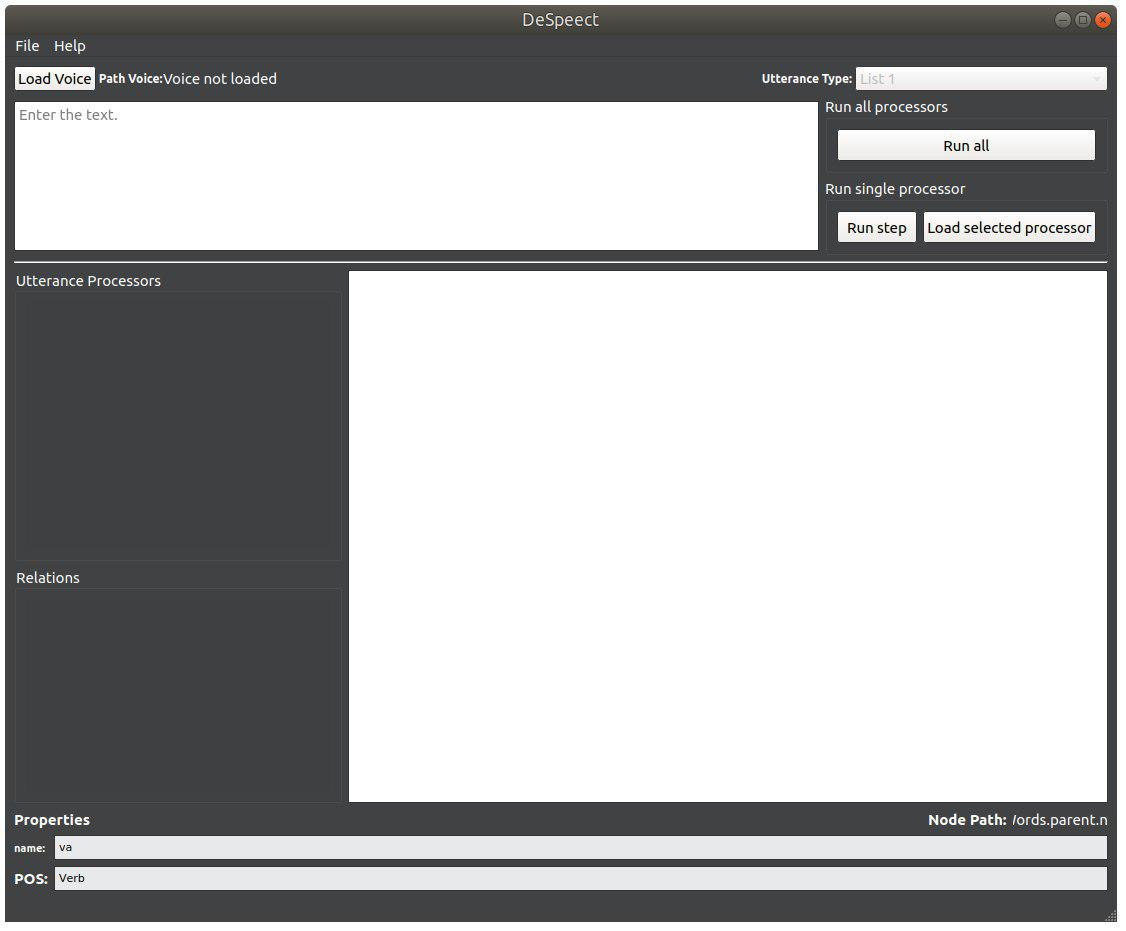
\includegraphics[width=\textwidth]{./img/avvio}
		
		\caption{Interfaccia grafica - Schermata iniziale}
	
	\end{figure}

	All'avvio dell'applicazione viene presentata una schermata come in Figura 4.1.\\
 	L'interfaccia grafica sarà sempre generalmente composta dalle seguenti componenti:
 	\begin{itemize}
 		\item \textbf{Menù dell'applicazione}: situato nella parte superiore della schermata, dal quale è possibile interagire con \textit{Speect} e con le funzionalità offerte dal sistema (vedi Figura 4.2);
 		\begin{figure}[H]
 			
 			\centering
 			
 			
\includegraphics[width=.3\textwidth]{./img/menu}
 			
 			\caption{Interfaccia grafica - Menù dell'applicazione}
 			
 		\end{figure}
 	
 		\item \textbf{Pannello di configurazione}: situato sotto il menù, nella parte superiore della schermata, dove è possibile caricare una voice, inserire input testuale, selezionare l'\glossario{utterance}{utterance} type e avviare l'esecuzione di \textit{Speect} eseguendo singolarmente ogni utterance processors o tutti assieme in una volta (vedi Figura 4.3);
 		\begin{figure}[H]
 			
 			\centering
 			
 			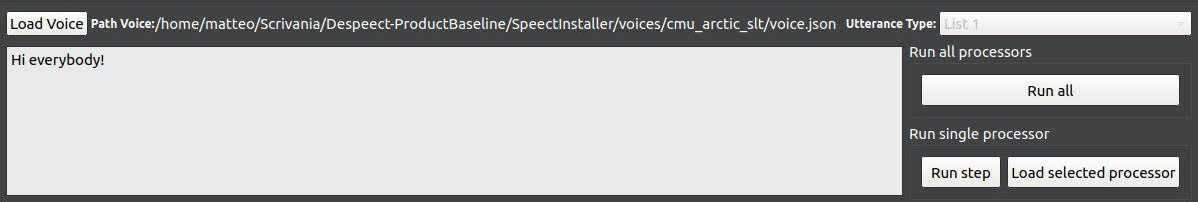
\includegraphics[width=\textwidth]{./img/pannello_configurazione}
 			
 			\caption{Interfaccia grafica - Pannello di configurazione}
 			
 		\end{figure}
 	
 		\item \textbf{Pannello degli Utterance Processors}: situato sulla sinistra appena sotto al pannello di configurazione, dove è possibile visualizzare ogni processor e capire quali sono stati eseguiti osservando le caselle relative sulla sinistra (vedi Figura 4.4);
 		\begin{figure}[H]
 			
 			\centering
 			
 				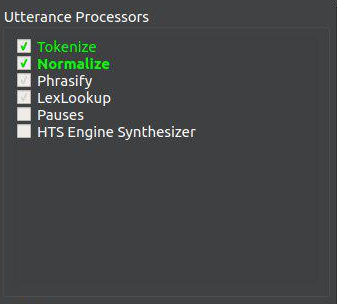
\includegraphics[width=.4\textwidth]{./img/pannello_processors}
 			
 			\caption{Interfaccia grafica - Pannello degli Utterance Processors}
 			
 		\end{figure}
 		
 		\item \textbf{Pannello delle Relations}: situato sulla sinistra sotto al pannello degli utterance processors dove è possibile visualizzare le relations presenti nel grafo. Qui l'utente può, deselezionando una \glossario{relation}{relation}, togliere i relativi nodi dal grafo (vedi Figura 4.5);
 		\begin{figure}[H]
 			
 			\centering
 			
 				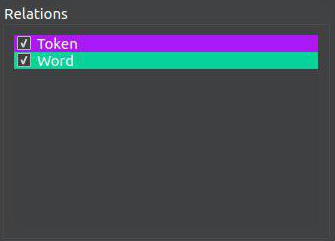
\includegraphics[width=.4\textwidth]{./img/pannello_relations}
 			
 			\caption{Interfaccia grafica - Pannello delle Relations}
 			
 		\end{figure}
 	
 		\item \textbf{Area del grafo}: situato sulla destra sotto al pannello di configurazione, dove viene visualizzato il grafo quando viene eseguito \textit{Speect}. I nodi sono selezionabili e si possono spostare (vedi Figura 4.6);
 		\begin{figure}[H]
 			
 			\centering
 			
 				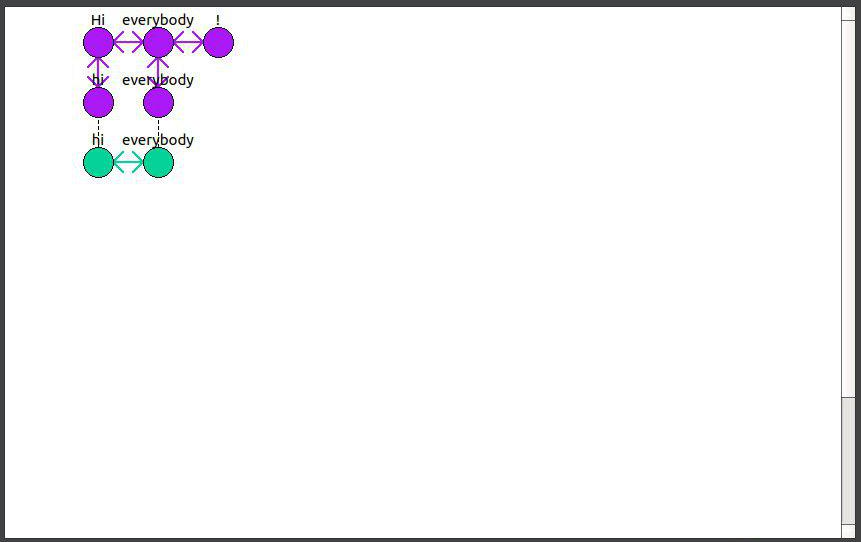
\includegraphics[width=\textwidth]{./img/area_grafo}
 			
 			\caption{Interfaccia grafica - Area del grafo}
 			
 		\end{figure}
 	
 		\item \textbf{Proprietà del nodo}: situato nella parte inferiore della schermata, dove vengono visualizzate le informazioni del nodo selezionato (vedi Figura 4.7).
 		\begin{figure}[H]
 			
 			\centering
 			
 				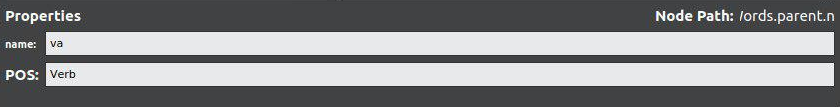
\includegraphics[width=\textwidth]{./img/proprieta_nodo}
 			
 			\caption{Interfaccia grafica - Proprietà del nodo}
 			
 		\end{figure}
 		
 	\end{itemize}
	
	\subsection{Menù dell'applicazione}
	Il menù è sempre disponibile in qualunque posizione vi troviate all'interno dell'applicazione e al suo interno è possibile selezionare le seguenti voci:
	\begin{itemize}
		\item \textbf{File} 
			\begin{itemize}
				\item \textbf{Save Voice JSon}: salva il file JSon;
				\item \textbf{Load HRG Graph}: carica un grafo HRG;
				\item \textbf{Save HRG Graph}: salva un grafo HRG;
				\item \textbf{Save Audio file}: salva il file audio prodotto in seguito all'esecuzione di \textit{Speect};
				\item \textbf{Search from path}: cerca un nodo inserendo come input un percorso specifico (es. Words.parent.n);
				\item \textbf{Exit}: chiude l'interfaccia \textit{DeSpeect};
			\end{itemize}
		
		\begin{figure}[H]
			
			\centering
			
				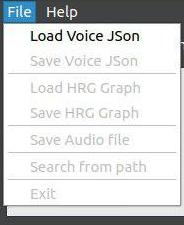
\includegraphics[width=.4\textwidth]{./img/menu_file}
			
			\caption{Menù dell'applicazione - Sezione "File"}
			
		\end{figure}
		\item \textbf{Help}
			\begin{itemize}
				\item \textbf{Manual}: apre il manuale utente;
				\item \textbf{Licence}: visualizza la licenza di \textit{DeSpeect}.
			\end{itemize}
	\begin{figure}[H]
		
		\centering
		
			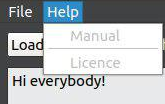
\includegraphics[width=.4\textwidth]{./img/menu_help}
		
		\caption{Menù dell'applicazione - Sezione "Help"}
		
	\end{figure}

	\end{itemize}
	
	\subsection{Visualizzare il manuale utente}
	Per visualizzare il manuale utente è sufficiente cliccare \textbf{Help} dal menù e selezionare la prima voce "Manual". 
	
	\subsection{Uscire dall'applicazione}
	Per uscire dall'applicazione è sufficiente cliccare \textbf{File} dal menù e selezionare l'ultima voce "Exit". 
	
	\section{Interagire con la voice}
	Questa sezione tratta l'utilizzo della voice, ovvero di un file JSon a partire dal caricamento fino a ciò che riguarda l'audio prodotto da \textit{Speect}.
	
	\subsection{Caricare la voice}
	Per caricare la voice è sufficiente cliccare \textbf{Load Voice}, pulsante situato nell'angolo in alto a sinistra del pannello di configurazione o in alternativa cliccare \textbf{File} dal menù e selezionare la prima voce "Load Voice".\\
	Una volta fatto ciò, si aprirà una finestra di ricerca del file browser dove cercare il file JSon. Una volta trovato basterà selezionarlo, cliccandoci sopra e cliccare \textbf{Apri}.\\
	A questo punto se verrà visualizzato il percorso del file JSon subito dopo "Path Voice", vicino al pulsante di caricamento voice, significa che il caricamento della voice ha avuto successo.\\
	Nel caso in cui il caricamento del file abbia avuto esito negativo, ripetere la procedura.
	
	\subsection{Generare l'audio relativo alla voice}
	Dopo aver caricato la voice, per generare l'audio relativo alla voice è sufficiente cliccare \textbf{Run all}. In questo modo verrà eseguito Speect che eseguirà tutti gli utterance processors, visualizzando il grafo risultante, la lista degli utterance processors e la lista delle relations.\\
	\'E possibile inserire un input testuale prima di procedere con l'esecuzione di \textit{Speect} e anche selezionare un diverso utterance type, nel caso fosse presente.\\
	\'E possibile anche eseguire ogni singolo utterance processor uno alla volta e vedere man mano come evolve il grafo. Per ulteriori dettagli si rimanda alla sezione 4.3.3.1 di questo manuale.
	
	\subsection{Salvare l'audio relativo alla voice}
	Uno volta eseguito \textit{Speect}, per salvare l'audio è sufficiente cliccare \textbf{File} dal menù e selezionare la voce "Save Audio file".\\
	Una volta fatto ciò, si aprirà una finestra di ricerca del file browser dove cercare la cartella in cui salvare il file. Una volta trovata basterà selezionarla, cliccandoci sopra, scrivere il nome del file nella barra di testo apposita e cliccare \textbf{Salva}.\\
	Il file audio prodotto avrà l'estensione .wav .
	
	\section{Stampare il grafo}
	Per stampare/visualizzare il grafo è necessario aver caricato una voice e aver eseguito \textit{Speect} tramite \textbf{Run all} o \textbf{Run step}.\\
	Se sono state fatte queste azioni, allora nell'area del grafo si dovrebbe visualizzare un grafo e a lato la lista degli utterance processors e delle relations.
	
	\subsection{Importare il grafo}
	Per importare un grafo è sufficiente cliccare \textbf{File} dal menù e selezionare la voce "Load HRG Graph".\\
	Una volta fatto ciò, si aprirà una finestra di ricerca del file browser dove cercare il file. Una volta trovato basterà selezionarlo, cliccandoci sopra e cliccare \textbf{Apri}.\\
	
	\subsection{Selezionare gli utterance processors}
	Nel pannello degli utterance processors è possibile interagire con i processors tramite le caselle di spunta a lato.\\
	Togliendo la spunta da un processor, esso non verrà eseguito da \textit{Speect}.
	
	\subsection{Visualizzare il grafo}
	Il grafo è visualizzato nell'area del grafo ed è composto da:
	\begin{itemize}
		\item \textbf{Nodi}: visualizzati tramite cerchi con sopra scritto il loro name, cioè quello a cui si riferiscono. Hanno diversi colori e la lista delle relations a lato funge da legenda, in questo modo si identificano i nodi relativi ad ogni relation;
		\item \textbf{Archi}: visualizzati tramite freccie direzionali che collegano due nodi. Anche gli archi sono di diversi colori e si rifanno alla lista delle relations a lato.
	\end{itemize}
	 
	\subsubsection{Visualizzare il grafo step-by-step}
	Eseguendo \textit{Speect} con \textbf{Run step} è possibile eseguire un utterance processor per volta e vederne il risultato sul grafo che ad ogni step si aggiorna aggiungendo nodi.
	
	\subsubsection{Visualizzare l'intero grafo}
	Eseguendo \textit{Speect} con \textbf{Run all} è possibile eseguire tutti gli utterance processors in una sola volta e vedere subito il grafo completo.
	
	\section{Interagire con il grafo}
	Questa sezione spiega come poter interagire col grafo spostando nodi e archi, togliendo i nodi e gli archi relativi a determinate relations e come esportare il grafo.
	
	\subsection{Esportare il grafo generato}
	Per esportare un grafo è sufficiente cliccare \textbf{File} dal menù e selezionare la voce "Save HRG Graph".\\
	Una volta fatto ciò, si aprirà una finestra di ricerca del file browser dove cercare la cartella in cui salvare il file. Una volta trovata basterà selezionarla, cliccandoci sopra, scrivere il nome del file nella barra di testo apposita e cliccare \textbf{Salva}.\\
	
	\subsection{Traslare elementi grafici}
	Questa sezione spiega come traslare gli elementi grafici che compongono il grafo, ovvero nodi e archi.
	
	\subsubsection{Traslare nodi}
	Per traslare i nodi è sufficiente cliccare tenendo premuto su di un nodo e spostando il cursore, posizionare il nodo dove si desidera all'interno dell'area del grafo.
	
	\subsubsection{Traslare archi}
	Quando si trasla un nodo, gli archi che sono coinvolti direttamente con quel nodo si adatteranno alla nuova posizione del nodo.
	
	\subsection{Interagire con le relation}
	Nel pannello delle relations è possibile interagire con le relations tramite le caselle di spunta a lato.\\
	Togliendo la spunta da una relation, i relativi nodi verrano tolti dal grafo e viceversa se si aggiunge la spunta, verranno aggiunti i relativi nodi al grafo.
	
	\chapter{Risoluzione dei problemi}
	
	\section{Errori in DeSpeect}
	
	In questa sezione viene fornito un elenco di tutti i possibili errori che si possono riscontrare utilizzando l’applicazione \textit{DeSpeect}:
	\begin{itemize}
		\item \textbf{E01 - ...}:l'utente visualizza un opportuno messaggio di errore nel caso in cui tenti di ...;
	\end{itemize}
	
	\subsection{Struttura dei codici di errore} 
	%Credo vada nelle norme di progetto
	
	\subsection{Log degli errori}
	
	\section{Problemi con il reperimento di Speect}
	
	\section{Segnalazione di bug}
	
	\textit{DeSpeect} potrebbe contenere bug o potrebbe essere desiderabile apportare modifiche e ampliamenti alle sue funzionalità. \\ È possibile segnalare malfunzionamenti o richieste di nuove funzionalità sotto forma di GitHub \glossario{issue}{issue} all’indirizzo:
	\begin{center}
		\url{https://github.com/graphiteSWE/DeSpeect}
	\end{center}
  oppure scrivendo direttamente all'indirizzo e-mail:
  \begin{center}
  	\url{graphite.swe@gmail.com}
  \end{center}
	
	\appendix
	
	\printglossary[style=glossaryStyle, nonumberlist]
	
\end{document}
